\documentclass[10pt,dvips]{article}
\usepackage{epsfig}
\usepackage{fancyheadings}
%\usepackage{twocolumn}
\usepackage{verbatim,moreverb,doublespace}
%\usepackage{rotate,lscape,dcolumn,array,rotating,latexsym}

\topmargin=-0.6in
\setlength{\oddsidemargin}{0.0 in}
\setlength{\textheight}{9.0in}
\setlength{\textwidth}{6.5in}
%\renewcommand{\thepage}{2}
\renewcommand{\baselinestretch}{1.0}
\renewcommand{\thesection}{\Roman{section}}
\renewcommand{\thesubsection}{\Alph{subsection}}
\renewcommand{\thesubsubsection}{\Alph{subsection}.\arabic{subsubsection}}


\pagestyle{fancy}
\lhead{}
\chead{\bf University of Rhode Island - CONFIDENTIAL}
\rhead{}
\lfoot{}
\cfoot{\thepage}
\rfoot{}


\begin{document}

\begin{center}
{\Large \bf University of Rhode Island}\\
{\Large \bf Invention Disclosure Statement}\\
\vspace{0.1in}
Augustus K. Uht - URI\\
David Morano - Northeastern University\\
David Kaeli - Northeastern University\\
January 12, 2000
\end{center}

\section{Description}
%\setcounter{subsection}{1}
\subsection{Invention Title}
{\bf ``Automatic and Transparent Hardware Conversion of
Traditional Control Flow to Predicates''}


\subsection{Description}
\label{desc}
This invention will increase the performance of
computers employing traditional control flow methods. The
cost is moderate and is much
less than competing techniques.
The control flow
conversion used {\it (CF-conversion)} is done transparently to the immediate
user of a computer. Such a user is normally either a compiler writer or an
assembly language programmer.

Performance is improved
by reducing the dependencies of machine instructions on each other, so
that more of the instructions can execute in parallel and hence reduce the
overall execution time of a program. Cost is reduced by accomplishing the
CF-conversion with relatively little hardware. Another major advantage
of the invention is its applicability to existing computer designs, including those
not having predicate operations in their machine instruction sets (such as the
common Intel x86 or IA-32 instruction set used in all Pentium microprocessors).

\subsubsection{Background}
The vast majority of computer programs use traditional control flow
constructs to determine when and if instructions in the program are
executed. Such constructs include {\tt if-then-else} statements and
various looping statements such as {\tt while(condition is true)\{ ... \}},
{\tt for(i initialized to 1; while i<10; increment
i every loop iteration)\{ ... \}} and {\tt do i=1 to 10 ... enddo}.
The vast majority of such control statements are realized with machine-level
instructions called {\it branches}, and most of these are {\it conditional} branches.

Branches are used as follows.
Most computers employ a model of computation using a pointer to the code of
the program it is executing; this {\it program counter} or PC contains
the address of the machine instruction the computer is currently executing. Every time
an instruction is executed, the default action is to increment the PC to point
to the next instruction to be executed. Most useful programs employ branches to
conditionally modify the contents of the PC to point to other places in a program, not
just the next instruction. Therefore a conditional
branch has the semantics: {\it if (condition
is true) then load the PC with a (specified) value}.

A well-known alternative to conditional branches is the use of {\it predicates}.
A predicate is typically a one-bit variable having the values true or false; it
is usually set by a comparison instruction. In this model every instruction has
a predicate as an additional input. The semantics is that the instruction is
only effectively executed (its output state changed)
if the predicate is true. An example of equivalent
classic control flow and modern predication follows.

\vspace{0.1in}
\begin{center}
\begin{minipage}{6.1in}
\begin{spacing}{1}
\begin{verbatimcmd}
       {\rm Classic code:}               {\rm Predicated code:}
1.  if (a==b) \{                1. Pred = (a==b);  //Pred set to true if a equals b.
2.      z=x+y;                 2. IF (Pred) THEN z=x+y; //Operations performed only
3.      w=a+b; \}               3. IF (Pred) THEN w=a+b; //    if Pred true.
4.  // later instructions:     4. // later instructions: NOT dependent on 1.
    //   all dependent on 1.
\end{verbatimcmd}
\end{spacing}
\end{minipage}
\end{center}
\vspace{-0.25in}

In traditional computers, all instructions following a branch are
dependent on the branch and must wait for the branch to execute before
executing themselves. This has been well-demonstrated to be a significant
barrier to realizing much parallelism within a program, keeping performance
gains low.

With predication, however, only the instructions having the equivalent
predicate as an input are dependent on the branch-remnant (the comparison
operation). In the example and in
general, this means the instructions after the predicated instructions are now
independent of the branch-remnant and may be executed in parallel with instructions
before the branch-remnant, improving performance.

Current approaches to using predication use {\it visible} and {\it explicit}
predicates; the predicates are controlled by the computer user and they use
storage explicitly present in the computer's instruction set architecture
(similar to regular data registers or main memory); they are explicit since
there is at least one 1-bit predicate hardware
register associated with each instruction.
The most extreme example of
this is the IA-64 (Intel Architecture-64 bits) architecture. The first
realization of this architecture is the Itanium (formerly Merced)
processor, due to be on
the market in the year 2000. Itanium has 64 visible-explicit predicate
registers\cite{Intel99}.
The predicates can not be effectively used when the processor executes
traditional IA-32 (x86) machine code. Therefore, billions of dollars of
existing software cannot take advantage of Itanium without modification.
Other types of microprocessors have similar constraints to x86 processors;
predicates are not currently in their instruction set, so they cannot take
advantage of predication techniques. 

It is possible to predicate just a subset of the instructions of a processor
but then the benefits of predication are much less. Therefore {\it full predication}
is preferred.

In prior work\cite{Uht85c,Uht86,Uht91} we devised a method for realizing an
equivalent to full predication called {\it minimal control dependencies} or
MCD.
It produced substantial performance gains\cite{Uht91,Uht92}, especially when
coupled with another performance-enhancing technique of ours called
{\it disjoint eager execution}\cite{Uht95}. MCD can be considered to have
{\it hidden} and {\it implicit} predicates, in that the predicates are not
visible to the user, nor are they explicitly present in the processor.
However, MCD has disadvantages when compared to predication
such as a high hardware cost (more logic gates and storage
needed) with relatively complex hardware. In particular, {\it j-by-j}
diagonal bit matrices are required, where {\it j} is the number of instructions
in the instruction window (those instructions currently under consideration for
execution by the processor). In a high-ILP machine, {\it j} might
be 256 or more, leading to a cumbersome 32,000 or more bit diagonal matrix.
Further, all of the bits need to be accessed and operated on at the same time,
leading to a very complex and potentially slow hardware layout. Lastly, setting
the contents of the matrix when instructions are loaded into the processor is
also costly and potentially slow.

The subject invention realizes the best features of both visible-explicit
predicates and hidden-implicit predicates without the disadvantages.

\subsubsection{The Invention}
{\it Hidden-explicit} predicates are realized by the invention; the predicates
are not visible to the user and thus may be implemented in any processor
architecture, and the predicates occupy explicit hardware register bits in the
processor, reducing cost and complexity. There are two parts to the invention:
the {\it predicate-assignment} part, taking place when instructions are loaded
into the processor, and the {\it predicate-use} part, taking place at instruction
execution time.

\paragraph{Nomenclature: } A branch's {\it domain} consists of the instructions
occurring between the branch and the branch's target. Thus, the branch controls the
execution of the instructions within its domain. If the branch's condition
evaluates true the branch is {\it taken}, and the instructions in its domain
are not executed. If the branch's condition evaluates false, the branch is
{\it not taken} and the instructions in the branch's domain are allowed to
execute.

Multiple branch domains can be arranged in an unlimited number of ways, all of
which are combinations of the three basic arrangements: {\it disjoint}, {\it nested}
and {\it overlapped}, as shown in Figure~\ref{branchcombos}. For full predication
all possible combinations of these arrangements must be handled correctly. The
invention does this.

\begin{figure}
\centering
\epsfig{file=brarrang.eps,height=2.50in}
\caption{{\em Branch arrangements.} Any system realizing full predication must be
able to handle any combination of these three basic branch arrangements.}
\label{branchcombos}
\end{figure}



\paragraph{Key Ideas: } The predicate-assignment hardware detects the beginnings
and ends of branch domains. The predicate-use hardware employs this information to
realize the beginnings and ends of domains at execution time, performing the
appropriate enabling and disabling of instructions in domains.

In general,
as each new domain is encountered during code execution, a new condition is
placed on the execution of the code within the new domain. If the branch condition
of the domain's branch is $bc_i$, and the predicate of the code \underline{before}
the branch is $p_r$, then the effective predicate $p_e$ of the new code in the new
branch's domain must be computed as: \[p_e = \overline{bc_i} \cdot p_r \]

When a domain is exited (upon reaching the corresponding branch's target instruction)
the effect of the corresponding branch must be nullified, in other words $bc_i$
should have no effect on the execution of the following code. This is achieved by
effectively OR-ing the opposite value of the branch condition with the current
predicate; in other words, the following is effectively computed for the code
after the branch domain:
\[p_{e2} = p_e + (bc_i \cdot p_r) = (\overline{bc_i} \cdot p_r) + (bc_i \cdot p_r) = p_r \]

This logic is realized by the combined operation of the predicate-assignment
and predicate-use hardware.

\subsubsection{Predicate-Assignment Hardware and Operation}
The function of the predicate-assignment hardware is to assign predicate and
{\it cancelling predicate} addresses to instructions as they are loaded into the
processor's load buffer and before the buffer contents are sent to the
instruction window for execution. The assignment is done by detecting
domain entries (branches) and exits (targets). The basic hardware structure
is a {\it branch tracking stack} or buffer
as shown in Figure~\ref{branchstack}. (We use the term
``stack'' in its generic sense; any kind of temporary storage may likely be used.)

\begin{figure}
\centering
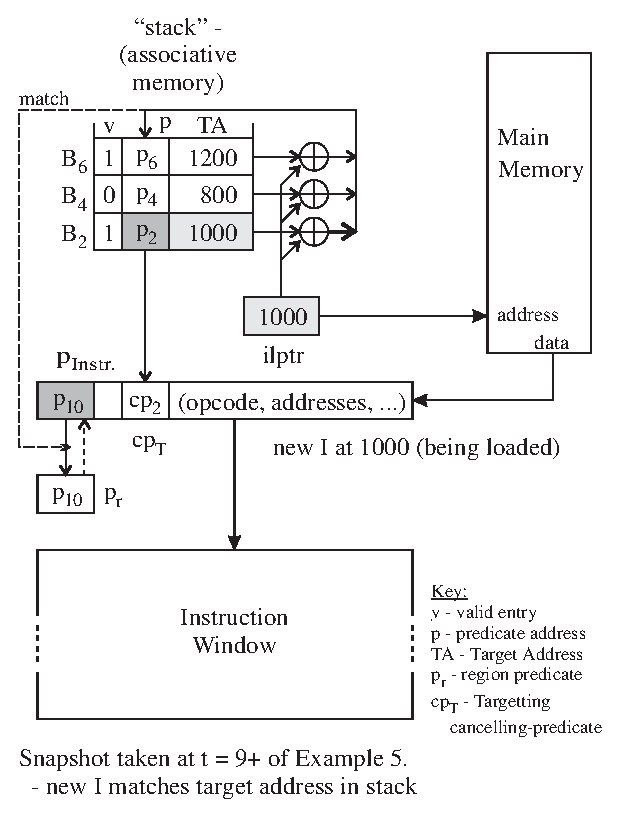
\epsfig{file=predasgn.eps,height=3.0in}
\caption{{\em Predicate-assignment hardware.}
The stack is associatively addressed by the current value of the $ilptr$ (instruction
load pointer). The predicate address of the branch corresponding to
a target address match with the $ilptr$ is output from the hardware and used to
augment the state of the instruction being loaded. The $p_r$ register holds the
address of the current region's predicate. $p_r$ may point to the predicate
from either a branch or a branch target.}
\label{branchstack}
\end{figure}

Each entry (row) in the stack corresponds to one branch. Typically, but not
necessarily, a branch is on the stack only while the instruction load pointer
$ilptr$ 
value is within the branch's domain. The following fields compose each entry:
\begin{enumerate}
\item address of predicate corresponding to the branch $p_b$
\item address of cancelling predicate corresponding to the branch $cp_b$; in practice
this may be derived from the branch's predicate address, so no explicit entry would
be needed for cancelling predicate addresses
\item target address of the branch $ta_b$
\item valid bit flag $v_b$; true while the target of the corresponding branch
has not yet been reached; the stack entry may be reclaimed and reused when the
valid bit is false
\end{enumerate}

A branch is placed on the stack when it is encountered by the $ilptr$ and is
removed when its target is reached. In the case of overlapped branches, the
target for a branch may be reached before a prior branch's target has been
reached; in this case the overlapped branch has its $v$ bit cleared and
is removed from the stack when convenient.

The comparators look for a match between the $ilptr$ and the target addresses.
If there is a match, it means that the instruction just loaded is the target
of the matching branch (multiple matches will be considered later). The
current cancelling predicate address $cp_T$ is set equal to the cancelling
predicate address of the matching branch. $cp_T$ is entered into the cancelling
predicate address field of the instruction being loaded.

\paragraph{Out-of-Bounds Branches: }
So far only branches with targets inside the window have been considered.
It is also possible that a branch in the window could jump to a point
not yet encountered by the predicate-assignment hardware. Therefore
the hardware shown in Figure~\ref{branshstack} is augmented
with some more circuitry to handle these 
{\it out-of-bounds} branches.
The new circuitry consists primarily of another set of comparators
for performing associative
lookups on field ``p''.

The technique is as follows. A candidate branch for execution supplies its
predicate address to the tracking buffer circuitry. The address is used
as a key
to perform a lookup on the ``p'' field.
If a branch's domain is wholly contained in the window, then the
branch will not have a valid entry in the buffer. Therefore if the candidate
branch does obtain a valid match, it is an out-of-bounds branch; further, the
branch's target address is then read from the corresponding TA tracking buffer
entry. The latter reduces storage costs, as target addresses need not be
stored in the window, and also simplifies operation because target addresses do
not need to be read from the window.

\subsubsection{Predicate-Use Hardware and Operation}
The Predicate-Use (PredU) hardware augments the state and operations of instructions
held in the processor's instruction window. None of the PredU hardware is visible
to the user, i.e., it does not appear in the processor's instruction set
architecture, and thus may be applied to any type of processor.

The overall effect of the PredU hardware is to chain predicate sources and sinks
so as to both enforce the functionality of the system and to keep the hardware
cost low. The alternative to chaining the predicates is to have very many predicate
inputs for each instruction, which would be costly in terms of additional
instruction state and therefore also more complex in operation.

The PredU hardware and operations differ depending on whether the instruction is
a branch or an assignment statement. Both cases are now considered.

\paragraph{Branch PredU Hardware and Operations: }
The output predicates are evaluated or re-evaluated whenever the input
predicate or branch condition becomes available or changes value, resp.
\begin{description}
\item[Input:] $p_r$ - predicate of region, same as input predicate $p_{in}$
\item[Outputs:] \[ \]
\vspace{-0.6in}\\
branch predicate: \[p_{out} = \overline{bc} \cdot p_r\] 
branch cancelling predicate: \[cp_{out} = bc \cdot p_r\]

$bc$ is the Branch Condition of
this branch. $bc$ has the values true (1) and false (0). It is set as the result
of some comparison test operation such as: $A < B$. The comparison may be performed
either as part of the branch's execution or as part of a prior instruction,
depending on the processor architecture.

\item[Execution Enabling Predicate:] Typically none. The branch executes
whenever its inputs are available or change value. Therefore all branches in the
instruction window may execute in parallel and out-of-order.
\end{description}

\paragraph{Assignment Statement PredU Hardware and Operation: }
Assignment statements also have predicate inputs and outputs.
These are used both for predicate-chaining and predicate-cancelling.
Recall that predicate-cancelling occurs when a branch domain is exited.

\begin{description}
\item[Inputs:] \[ \]
\vspace{-0.6in}\\
$p_r$ - predicate of region; same as input predicate $p_{in}$\\
$cp_T$ - cancelling predicate of targeting branch, if any; same as $cp_{in}$

\item[Output:] \[p_{out} = p_r + cp_T = p_{in} + cp_{in}\]

$p_{out}$ is computed independently of the rest of the assignment statement's
execution and computations.

\item[Execution or Assignment Enabling Predicate:] $p_I$ - same as output:
\[p_I = p_{in} + cp_{in}\]

The assignment instruction may modify its traditional sinks when $p_I$ is true.
Such sinks are the results of the regular operations of the assignment statement,
e.g., if the instruction is: $A = B + C$ then $A$ is a traditional sink and is
written if the instruction's predicate evaluates true.
\end{description}

\subsubsection{Special Case: Multiply-Targeted Instructions}
There is a not-so-special case that can often arise in code and that we have not
yet addressed. This is the case when an instruction is the target of more than
one branch. In this scenario the hardware as described so far will not work, it
is only suitable for an instruction being the target of no more than one branch.

There are two orthogonal solutions that can be employed to handle the
multiple-target case. The first is to provide multiple cancelling predicate fields
for each instruction. This will cost more, but may be suitable for a small number
of cancelling predicates. However, we must handle the case when an instruction
is the target of many, many branches (this is possible in many machines, although
perhaps not likely).

The second solution is to insert a dummy No-Op instruction into the window after the
current instruction if the instruction runs out of cancelling predicate fields.
The No-Op's cancelling predicates can then be used in addition to the original
instruction's. Since any number of No-Ops can be
inserted, any number of branches targeting the same instruction can be
handled. Of course, a price is paid for a ``wasted'' slot in the instruction
window for each No-Op instruction added.

Experimentation is needed to determine a suitable number of cancelling
predicate fields for one instruction. It is likely that both solutions will
be used in a typical processor.

\subsubsection{Special Case: Branch is a Target of Another Branch}
It is also quite possible if not likely that code will contain a branch that
is the target of another branch. This scenario is readily handled by employing
all of the predicate and cancelling predicate logic in the branch, such that it
appears as BOTH a branch and an assignment statement. The cancelling predicate
output of such an instruction is the same as that of an un-targetted
version of the branch. The
predicate output combines the functions of the branch predicate and the
assignment statement predicate, with the branch portion using
the assignment portion as its region predicate input:
\[p_{out} = \overline{bc} \cdot (p_r + cp_T) = \overline{bc} \cdot (p_{in} + cp_{in}) \]
This works because the assignment portion effectively (logically) takes place
before the branch.

\subsubsection{Examples}
We now present four examples to illustrate the operation of the hidden-explicit
predicate system. The examples cover the following cases:
\begin{enumerate}
\item Two disjoint branches, Figure~\ref{predex_d}. (Also covers the cases of straightline code and a single branch.)
\item Two nested branches, Figure~\ref{predex_n}.
\item Two overlapped branches, Figure~\ref{predex_o}.
\item Three branches with a combination of nesting and overlapping, Figure~\ref{predex_c}.
\end{enumerate}

All of the examples have the same format. In the code column: ``I'' instructions are
assignment statements, and ``B'' instructions are branches. The branch domains are
shown with arrowed lines. Each example can be followed by first going down the
{\it predicate-assignment} table entries, in order, as the instructions would
be loaded. Using the tracking stack, this results in the predicate addresses shown
in the $p_{in}$ and $cp_{in}$ columns being generated and entered into the corresponding
instruction's fields in the instruction window.

Next, the predicate-use table entries may be examined to see how the predicates
are evaluated at run-time, how their values are chained and how branch domains
are effectively exited. For an example of the latter, refer to Figure~\ref{predex_d}
and look at the $p_I$ entry for the assignment instruction at address 400.
Although it has predicate inputs, their values cancel each other out, $p_I$
is effectively ``1'' and thus the instruction is always enabled for
execution, as far as branches are concerned. This is correct, since it is
outside the domains of all of the branches in the code example.

\begin{figure}
\centering
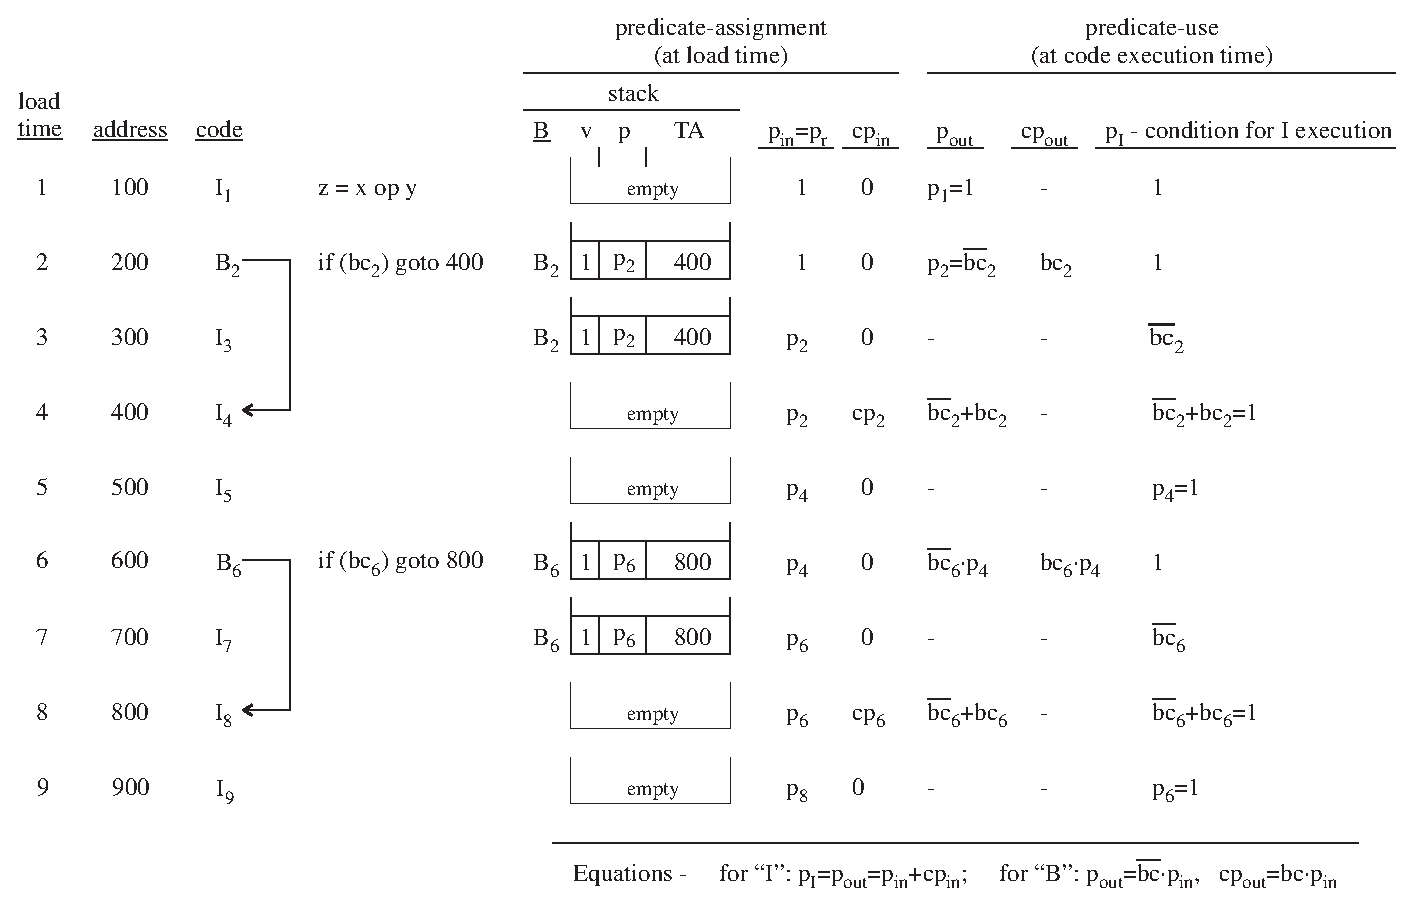
\epsfig{file=predex_d.eps,width=6.50in}
\caption{{\em Hidden-explicit predication example: \underline{disjoint branches}.} }
\label{predex_d}
\end{figure}

\begin{figure}
\centering
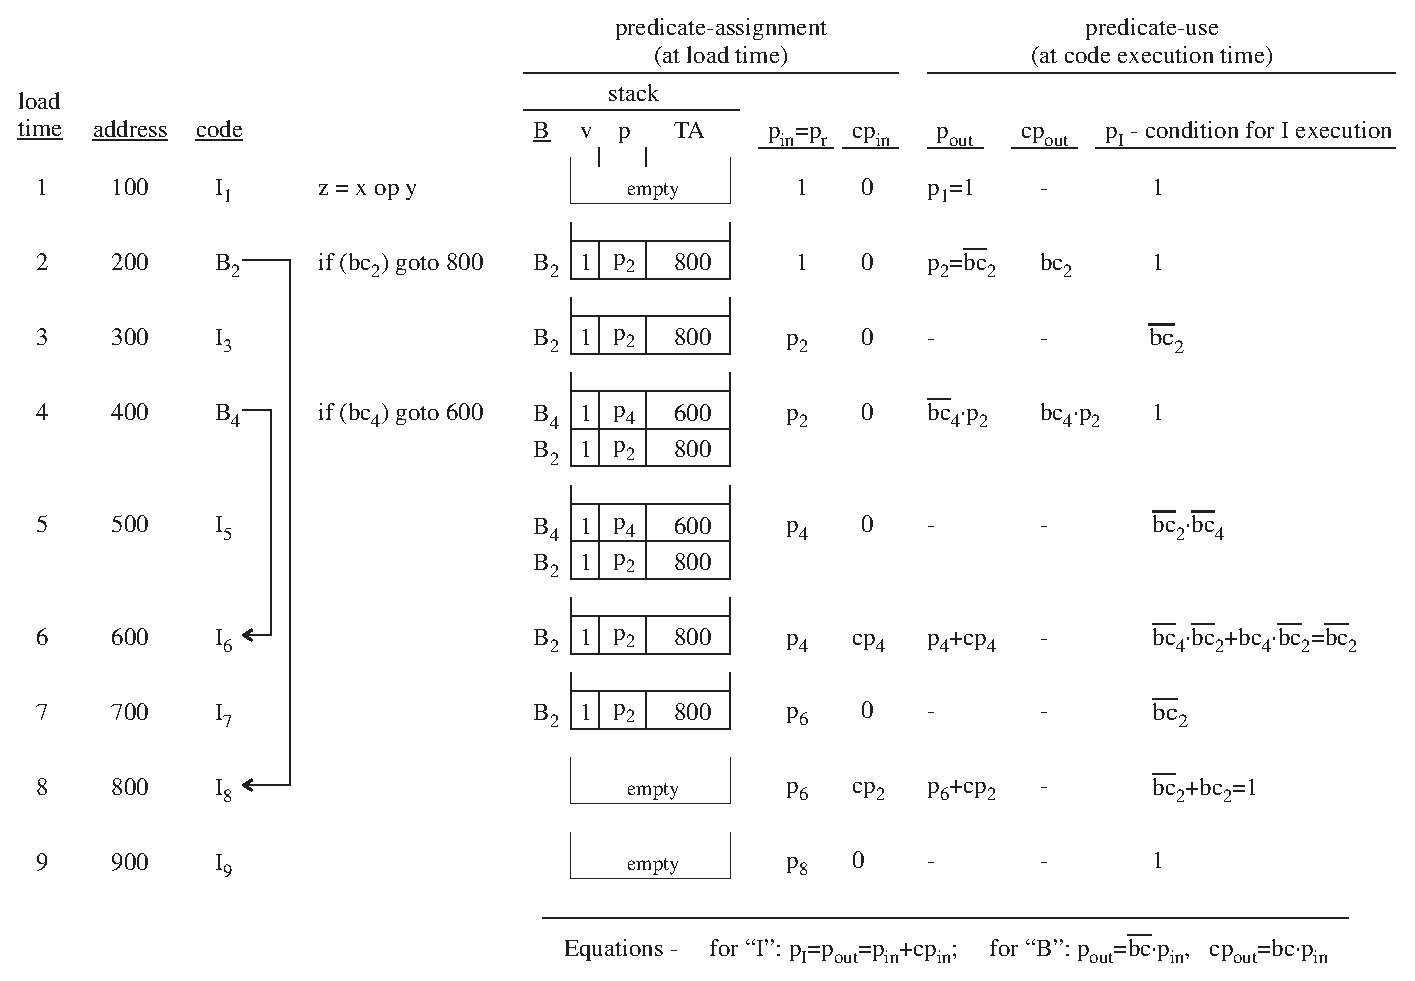
\epsfig{file=predex_n.eps,width=6.50in}
\caption{{\em Hidden-explicit predication example: \underline{nested branches}.} }
\label{predex_n}
\end{figure}

\begin{figure}
\centering
\epsfig{file=predex_o.eps,width=6.50in}
\caption{{\em Hidden-explicit predication example: \underline{overlapped branches}.} }
\label{predex_o}
\end{figure}

\begin{figure}
\centering
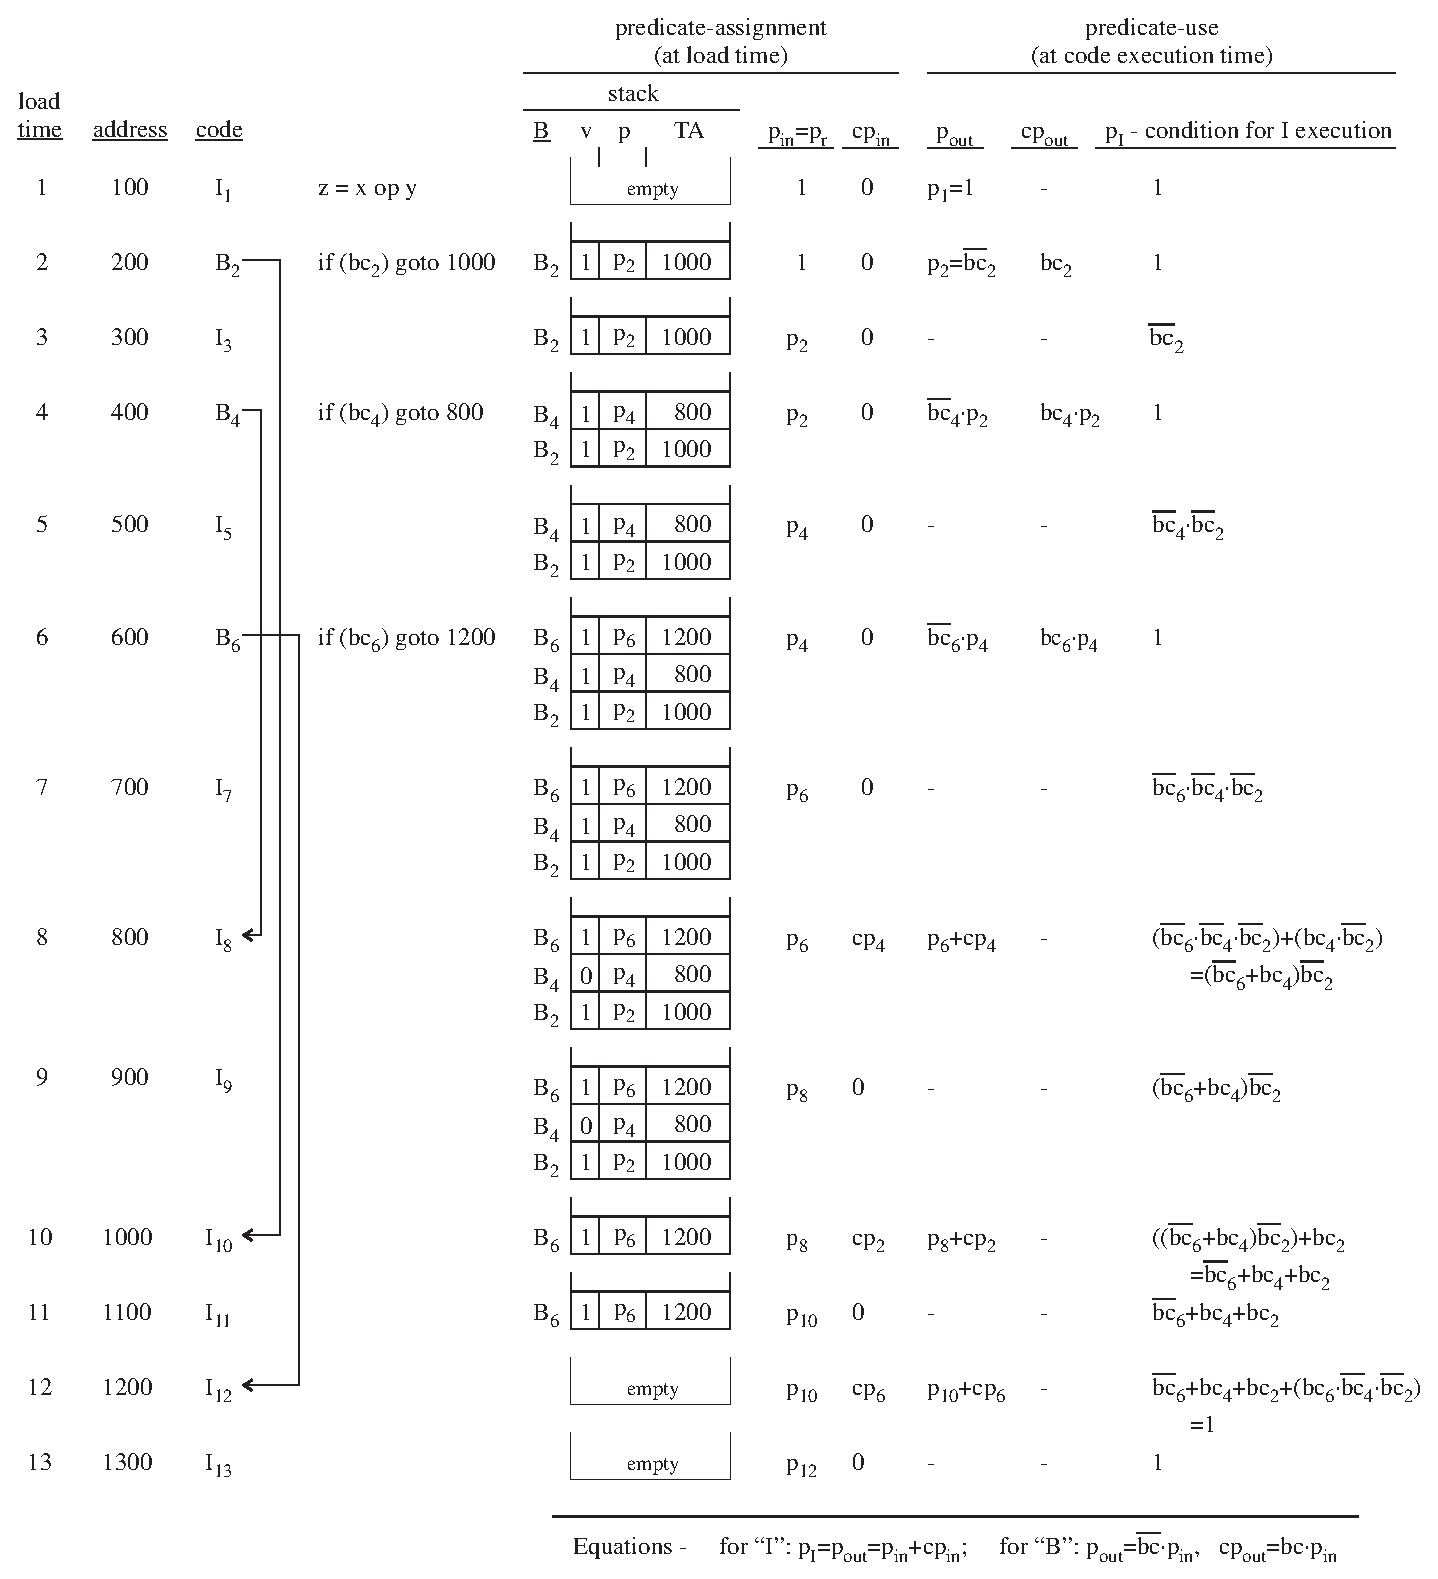
\epsfig{file=predex_c.eps,width=6.50in}
\caption{{\em Hidden-explicit predication example: \underline{mixed branches}.} }
\label{predex_c}
\end{figure}

\subsubsection{Prior Work and Alternate Solutions}
\label{priorwork}
\paragraph{Comparison to Traditional Systems: }
As discussed earlier, hidden-explicit predication allows more parallelism than
traditional purely branch-based processors. 

\paragraph{Prior Work}
Reduced control dependencies were originally studied in \cite{Tjaden72}.
Minimal control dependencies were built on this model and were fully devised in
\cite{Uht85c,Uht86,Uht91}. The latter, also used in \cite{Uht95}, required
large and potentially complex domain and/or dependency matrices.
Visible-explicit predication first appeared
as ``guards''
in the supercomputing field in the 1960's and '70's.
A limited form
of hidden-explicit predication is presented in \cite{Klauser98}, but it is not
truly hidden in that the compiler must delineate the domains. It also only
predicates branches 
not part of nested or overlapped branch domains,
relying on standard branching techniques
for other branches. Our method allows full predication.

To our knowledge, our approach is unique. 

%\subsubsection*{References}
\bibliographystyle{ieeetr}
\bibliography{cdgnew}


\subsection{Is this a new invention, different enough from any other invention,
including any that you may have previously disclosed, that it will carry new
claims?}
Yes. 

\subsection{What is the invention?}
It is a combination of: a new process, a new device, one or more new
products, and a new use for or
an improvement to an existing product or process.

\subsection{What are the immediate and/or future applications of the invention?}
Improving the performance of any traditional computer.
It is likely to be applicable over the
life of the patent, i.e., in both the short and the long term. Immediate application.

\subsection{Why is the invention better -- more advantageous -- than present technology?}
It allows traditional processor designs to execute instructions after branches
independently of the branches, enhancing parallelism and hence improving performance.
This is achieved with substantially less cost and complexity than prior inventions.

\subsection{What are its novel and unusual features?}
The notion of a ``cancelling predicate'' is completely novel, to our knowledge.
The use of a stack to assign predicate addresses is novel. The chaining of
predicates is novel. The use of assignment statements to help realize the function
of the branches is novel.

\subsection{What problems does it solve?}
The eternal quest for more performance, preferably at little cost.

\subsection{How does the invention differ from present technology?}
There are two classes of processors in present or soon-to-be-present technology.
The invention improves upon both in different ways. The first class of processors
is the traditional class in which there is little or no predication. In these
processors all instructions after a branch are dependent on the branch, constraining
performance; the invention reduces this constraint. Traditional processors also
cannot be retrofitted with predicates as currently defined, since this would
require a change in the processor's instruction set, making it incompatible with
existing code.

The second class of processors is a newly-emerging class in which the predicates
are explicit and present in the instruction set of the processor (visible); e.g., the
Intel Itanium, to appear on the market
in the year 2000. Since the predicate structure
is visible, it cannot be easily changed. For example, if more predicates are
needed, they cannot be readily added to the processor for code-compatibility
reasons. It is also cumbersome to predicate instructions when they depend
on multiple branches. This normally takes extra instructions, since each Itanium
instruction can be guarded with only one predicate register.
With the invention, an unlimited number of predicates may be added
without affecting the processor's instruction set and it is easy to
predicate an instruction on many branches. In fact, the latter is automatic
in the invention, not needing any compiler assistance.

\subsection{What problems does it solve or what advantage does it possess?}
See above.

\subsection{Is work on the invention continuing?}
Yes. It is being realized in the microarchitecture of a research machine called Levo.
A revised version of the Levo simulator is under construction at Northeastern
University under Prof.\ Uht's and Prof.\ Kaeli's
direction. We eventually plan to build a Levo prototype.

\subsection{Are there limitations to overcome or other tasks to be done prior to
practical application?}
Nothing essential, although it would be helpful and desirable to run simulations
to characterize the invention's contribution to processor performance. We are
planning to do this.

\subsection{Are there any test data?}
There is indirect test data. The effects of reduced and minimal control dependencies
have been studied before\cite{Uht95,Lam92}, showing large potential gains.
However this particular solution has not been tested or its performance measured.

\subsection{Have products, apparatus or compositions, etc., actually been made and tested?}
No.

\subsection{What disadvantages or limitations does the invention possess?
Can they be overcome? How?}
The invention uses more hardware than original processors
but not a substantially larger amount, especially
given current hardware density trends (the number of transistors on a chip doubles
avery 18 months - Moore's Law). The predicate-assignment portion of the hardware
is a potential performance bottleneck, but we believe it can be overcome. We will
measure its effect during the Levo simulations.

\subsection{Background: What is the field or art to which the invention applies?}
Computer central processing unit design.

\subsection{Does....earlier dated record of invention exist? Describe.}
Yes. In my research notebooks, which I carry with me. The invention was created
over a period of time, beginning on June 21, 1999 and ongoing, with major parts of
the invention created on October 5, 1999 and November 12, 1999. The corresponding
notebook entries were not countersigned until November 29, 1999. I have included
copies of the main sections.

\subsection{What do you see as the commercial value of your invention?}
Potentially large, since it is applicable to all computer processor designs.

\subsection{What firms may be, or are interested, and why?}
I have not approached anyone about this invention. A list of all
existing computer
companies would form the firms potentially interested in the invention, in particular those
focusing on high performance, both absolutely or with low-cost.
This would be to improve their product lines
and make them more competitive.

Example firms: AMD, IBM, Intel, Hewlett-Packard, ..... AMD might be very interested,
because they are keen to gain more market share from Intel. Intel tends to be
an NIH company (Not Invented Here), but not absolutely.

\newpage

\section{Publications, Public Use and Sale}
\subsection{Has invention been disclosed in an abstract, paper, talk, news story, or
a thesis?}
No.

\subsection{Is a publication or other disclosure planned in the next six months?}
Yes, one or more.

We plan on submitting one paper in June, 2000 to the International Symposium on
Microarchitecture. 

\subsection{Has there been any public use or sale of products embodying the invention?}
No.

\subsection{Are you aware of related developments by others?} Yes. See above.

\newpage

\section{Sponsorship}
WAS THIS RESEARCH SPONSORED?	YES.

\subsection{Government Agency: Yes}
This research was sponsored by the National Science Foundation under grants
MIP-9708183, EIA-9729839 and DUE-9751215. I am the Principal Investigator for
all of these grants.

\subsection{URI or Northeastern University:} No.

\subsection{URI Foundation:} No.

\subsection{Private Industry:} No.

\subsection{Has the invention been disclosed to industry representatives?} No.

\newpage

\section{For Our Records}

\subsection{Names and titles of inventors:}

\begin{verbatim}
Associate Professor Augustus K. Uht, URI, lead inventor

Signature:

Date:



Graduate Student and Doctoral Candidate David Morano, Northeastern University, inventor

Signature:

Date:



Associate Professor David Kaeli, Northeastern University, inventor

Signature:

Date:


\end{verbatim}

\subsection{Contact for more data:} Augustus K. Uht, x4-5431, uht@ele.uri.edu

\subsection{Mailing Address for lead inventor:}

\begin{verbatim}
Augustus K. Uht
44 Torrey Rd.
Cumberland, RI 02864-1220
\end{verbatim}

\subsection{Name and title of institutional representative:}

\begin{verbatim}

Signature:

Date:

Quentin C. Turtle, Director
Industrial Research and Technology Transfer

The Research Office
University of Rhode Island
70 Lower College Road, Suite 2
Kingston, RI 02881

Tel.   (401) 874-2304
FAX    (401) 792-9089
\end{verbatim}

\end{document}

